\documentclass[12pt]{article}
\usepackage{fontspec}
\usepackage[utf8]{inputenc}
\setmainfont{Bodoni 72 Book}
\usepackage[paperwidth=17in,paperheight=11in,margin=1in,headheight=0.0in,footskip=0.5in,includehead,includefoot,portrait]{geometry}
\usepackage[absolute]{textpos}
\TPGrid[0.5in, 0.25in]{23}{24}
\parindent=0pt
\parskip=12pt
\usepackage{nopageno}
\usepackage{graphicx}
\graphicspath{ {./images/} }
\usepackage{amsmath}
\usepackage{hyperref}
\usepackage{tikz}
\newcommand*\circled[1]{\tikz[baseline=(char.base)]{
            \node[shape=circle,draw,inner sep=1pt] (char) {#1};}}

\begin{document}

\begingroup
\begin{center}
\huge NOTES TO THE INTERPRETERS
\end{center}
\endgroup

\begingroup
\large \textbf{\circled{I} GENERAL:} \\
\normalsize \circled{1} \circled{a} After temporary \textbf{accidentals}, cancellation marks are printed also in the following measure (for notes in the same octave) and, in the same measure, for notes in other octaves, but they are printed again if the same note appears later in the same measure, except if the note is immediately repeated. \\
\circled{b} \textbf{Quartertones} are indicated using the following accidentals: \\
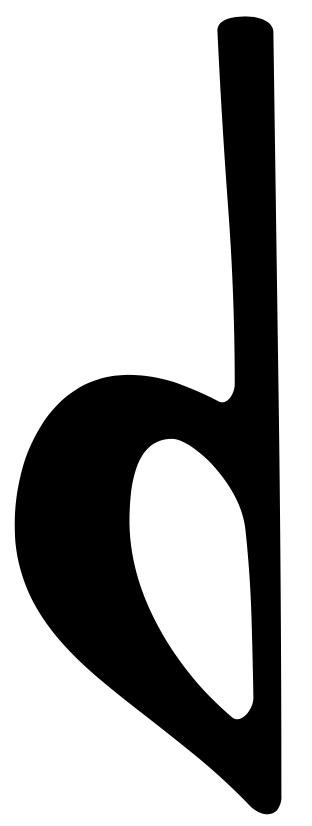
\includegraphics[scale=0.07]{qt_flat.png} A quartertone \textbf{flat} \\

\includegraphics[scale=0.07]{qt_sharp.png} A quartertone \textbf{sharp} \\
\circled{2} \textbf{Dashed, hooked lines} indicate that a playing technique should be \textbf{sustained}, whereas \textbf{solid lines with arrows} indicate a \textbf{gradual transition} from one playing technique to another. \\
\circled{3} This score follows the notational example of Luigi Nono, who used the familiar, round-arched \textbf{fermata} as an orientation point. To \textbf{triangulate} the arch indicates to \textbf{shorten} the fermata, and to \textbf{square} the arch indicates to \textbf{lengthen} the fermata. The \textbf{addition of arches} increases the relative length or shortness of the fermata. Interpreters are discouraged from developing a timing system for counting the relative length of the fermate. A fermata should be taken as an invitation to wait rather than to count, the shape of the symbol indicating the breadth of the waiting space. \\
\endgroup

\begingroup
\large \textbf{\circled{II} NOTE HEADS:}\\
\normalsize \circled{1} \textbf{Finger pressure of the left hand} is indicated with \textbf{note head shapes} as follows: \\
\circled{a} 
\includegraphics[scale=0.05]{harmonic.png} Harmonic pressure (These note heads will be coloured in if they are attached to quarter notes. Otherwise, they are transparent.) \\
\circled{b} 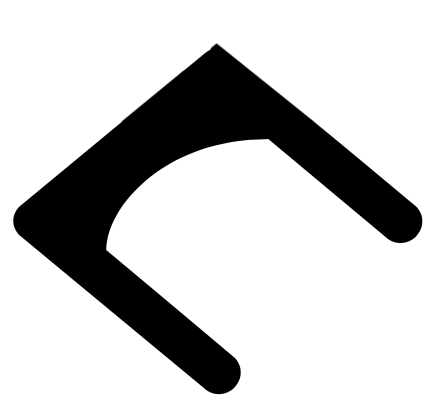
\includegraphics[scale=0.065]{half_harmonic_half_note.png} Half harmonic pressure (half notes and larger durations) \\
\circled{c} 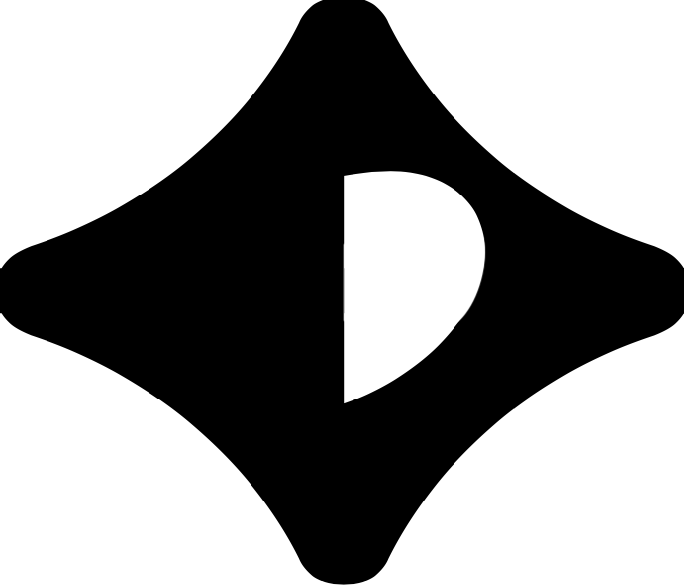
\includegraphics[scale=0.05]{half_harmonic_quarter_note.png} Half harmonic pressure (quarter notes and smaller durations) \\
\circled{d} 
\includegraphics[scale=0.05]{cross.png} Percussive or unpitched actions \\
\circled{2} \textbf{Transitions between finger pressures} are indicated using arrows between note heads, as below: \\
\begin{center}
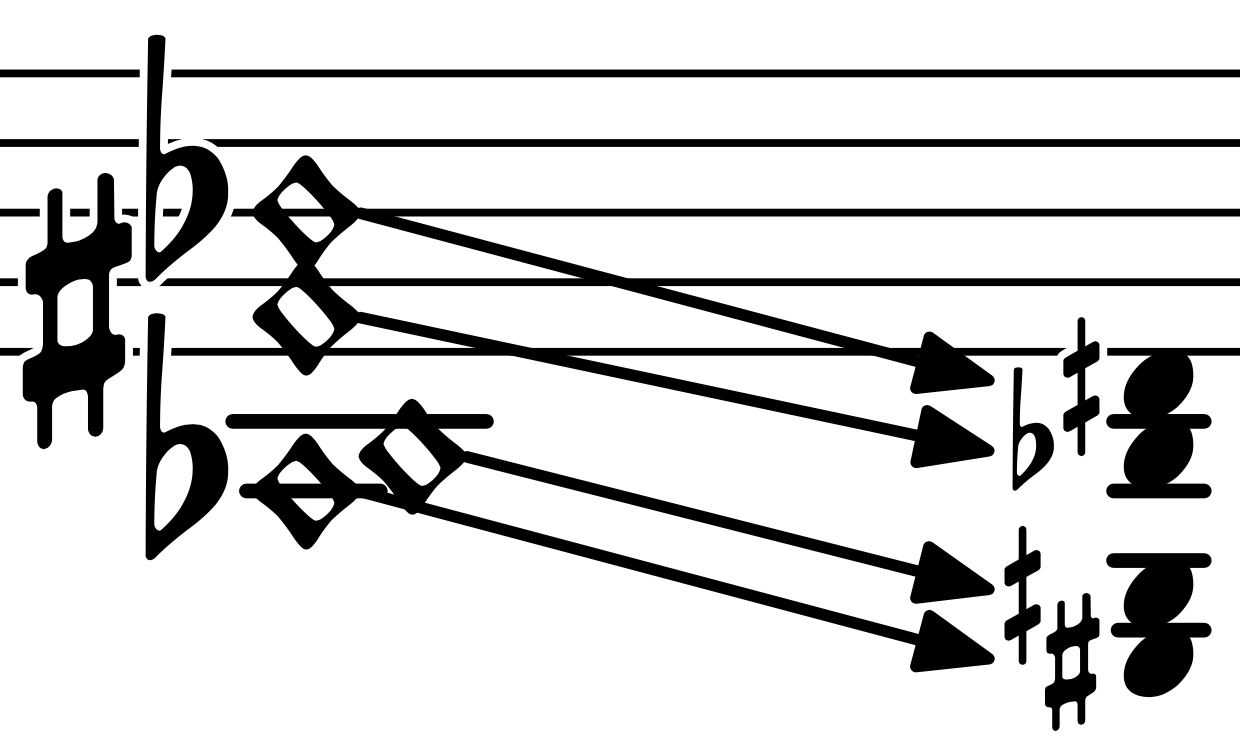
\includegraphics[scale=0.20]{in_staff_arrows.png}
\end{center}
These arrows \textbf{double as glissandi} when spanning between two different pitches. \\

\pagebreak

\circled{3} \textbf{Multiple muting} of the string is accomplished by \textbf{fingering two or more places on the same string at once.} This is indicated with \textbf{small, blue note heads} beneath the upper node, as below: \\
\begin{center}
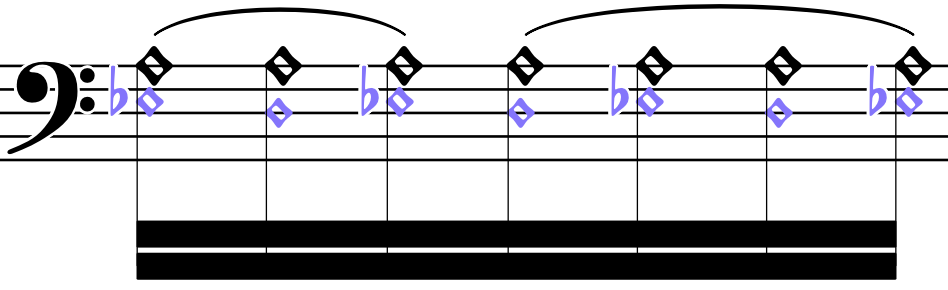
\includegraphics[scale=0.35]{multi_muting.png}
\end{center}
\endgroup

\begingroup
\large \textbf{\circled{III} STAVES AND CLEFS:} \\
\normalsize \circled{1} 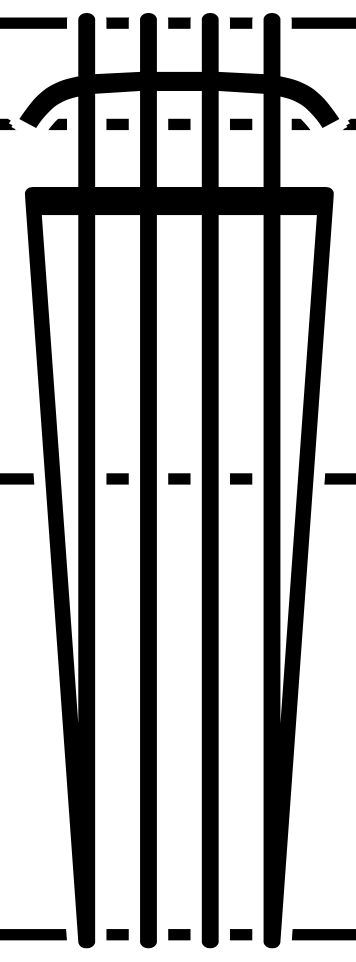
\includegraphics[scale=0.15]{tab_clef.png} A \textbf{four-line staff} wherein the top line indicates to play \textbf{behind the bridge}, the next to play \textbf{on the bridge}, the next to play at the \textbf{center of the fingerboard}, and the next to play at the \textbf{bottom of the fingerboard}, near the nut. \\
\circled{1} 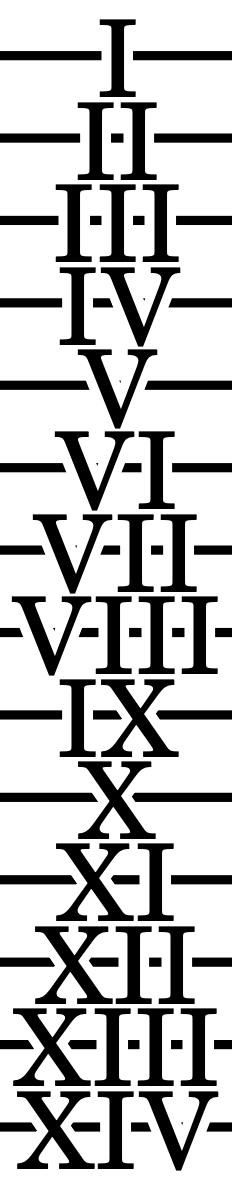
\includegraphics[scale=0.15]{string_clef.png} A \textbf{seven-line staff} (for viola da gamba) or a \textbf{fourteen-line staff} (for theorbo) wherein the \textbf{top line} indicates to play on \textbf{string I}, the \textbf{next line} on \textbf{string II}, and so on. \\
\endgroup

\begingroup
\large \textbf{\circled{IV} ABBREVIATIONS:} \\
\normalsize \circled{1} \textbf{dp.} = Dietro ponticello (play on the strings behind the bridge) \\
\circled{2} \textbf{ob.} = On the bridge (play directly on the bridge) \\
\circled{3} \textbf{xp.} = Extreme sul ponticello (play with half of the right hand implement directly on the bridge, and the other half on the string) \\
\circled{4} \textbf{msp.} = Molto sul ponticello (play very close to the bridge) \\
\circled{5} \textbf{p.} = Sul ponticello (play near the bridge) \\
\circled{6} \textbf{ord.} = Ordinario (cancels right hand contact point instructions) \\
\circled{7} \textbf{t.} = Sul tasto (play near the fingerboard) \\
\circled{7} \textbf{mst.} = Molto sul tasto (play above the edge of the fingerboard) \\
\circled{8} \textbf{xt.} = Extreme sul tasto (play with the right hand as close to the left hand as possible) \\
\circled{9} \textbf{rasg.} = Rasgueado \\
\circled{10} \textbf{Scratch} = Scratch tone (play with enough right hand pressure to remove as much pitch from the sound as possible) \\
\circled{11} \textbf{Norm.} = Normale (cancels right hand pressure instructions) \\
\circled{12} \textbf{CLT} = Col legno tratto \\
\circled{13} \textbf{CLB} = Col legno battuto \\
\circled{14} \textbf{LH/RH} = Right hand/Left hand \\
\endgroup

\begingroup
\large \textbf{\circled{V} VIOLA DA GAMBA:} \\
\normalsize \circled{1} Two \textbf{finger-pressure trills} appear in the piece. They are: \\
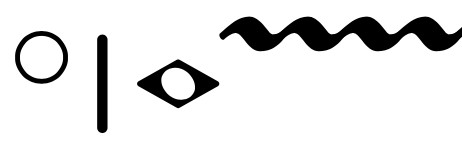
\includegraphics[scale=0.35]{open_mute_trill.png} between open string and harmonic pressure, and \\
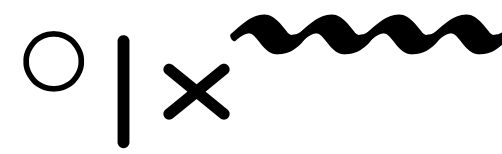
\includegraphics[scale=0.35]{open_perc_trill.png} between open string and percussive pressure. \\
\circled{2} \\
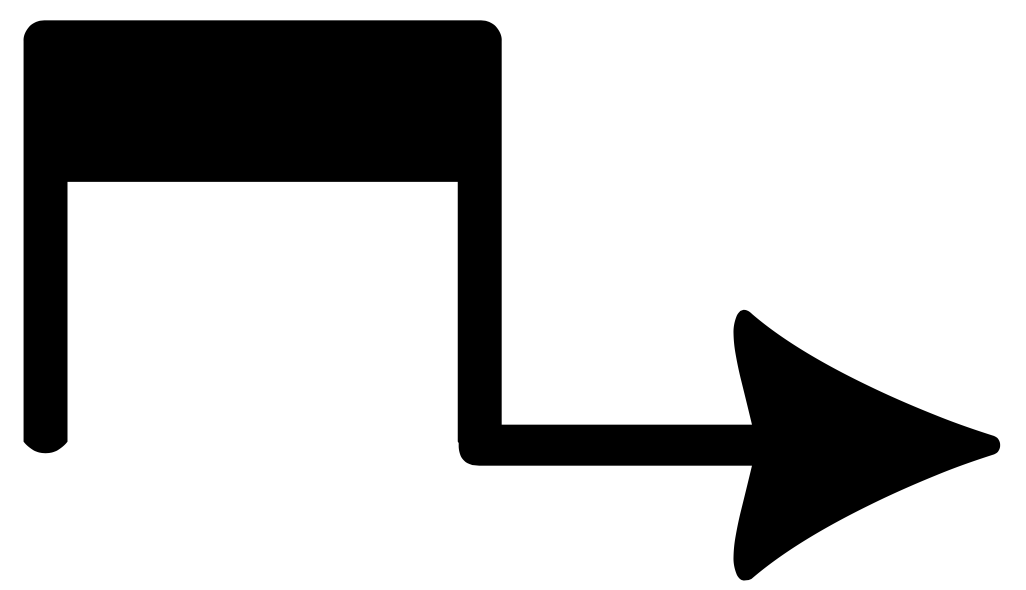
\includegraphics[scale=0.05]{talon_punta.png} Indicates to draw the bow evenly from \textbf{au talon} to \textbf{punta d'arco} over the duration of the articulated note. \\
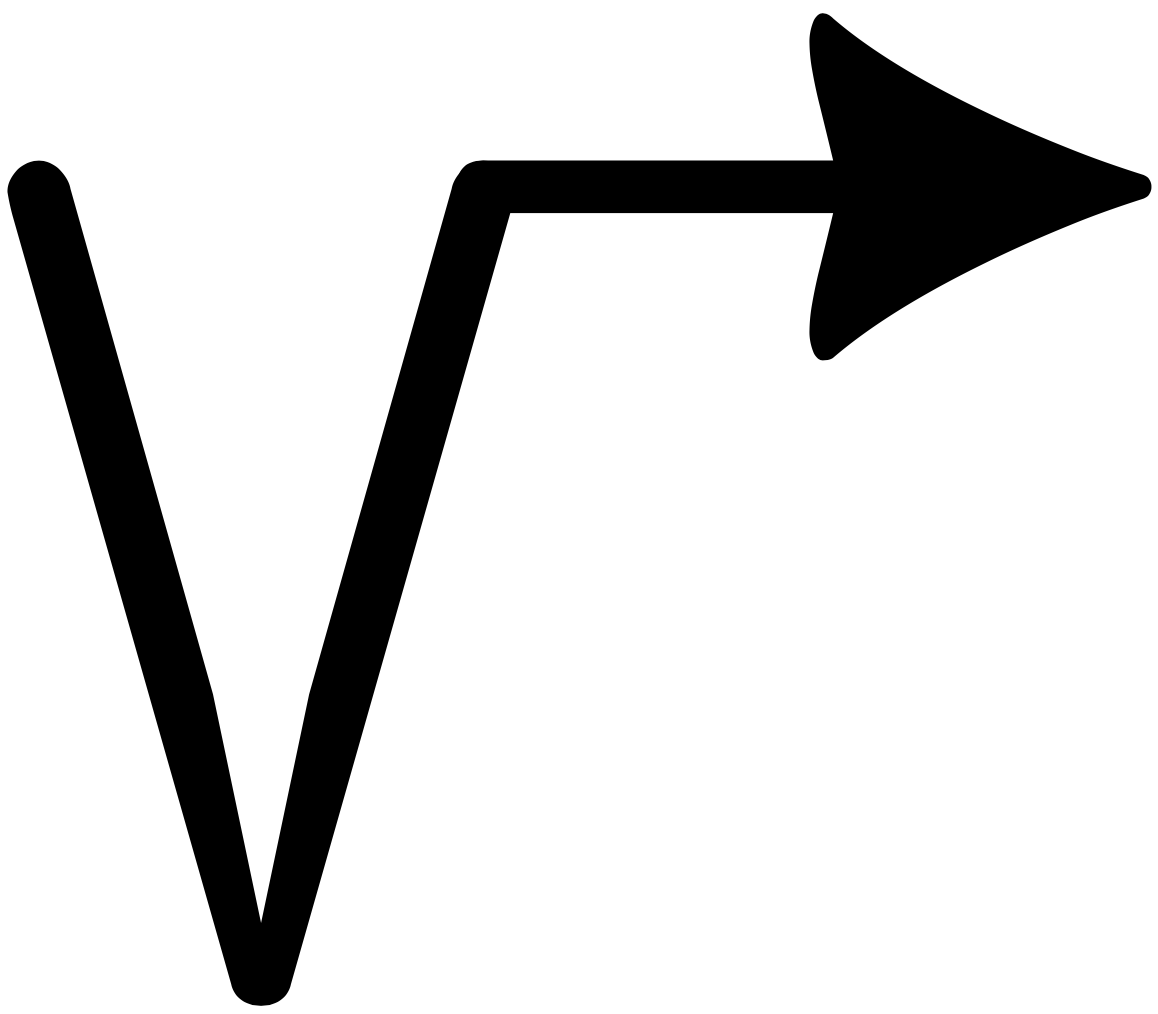
\includegraphics[scale=0.04]{punta_talon.png} Indicates to draw the bow evenly from \textbf{punta d'arco} to \textbf{au talon} over the duration of the articulated note. \\
\circled{3} \\
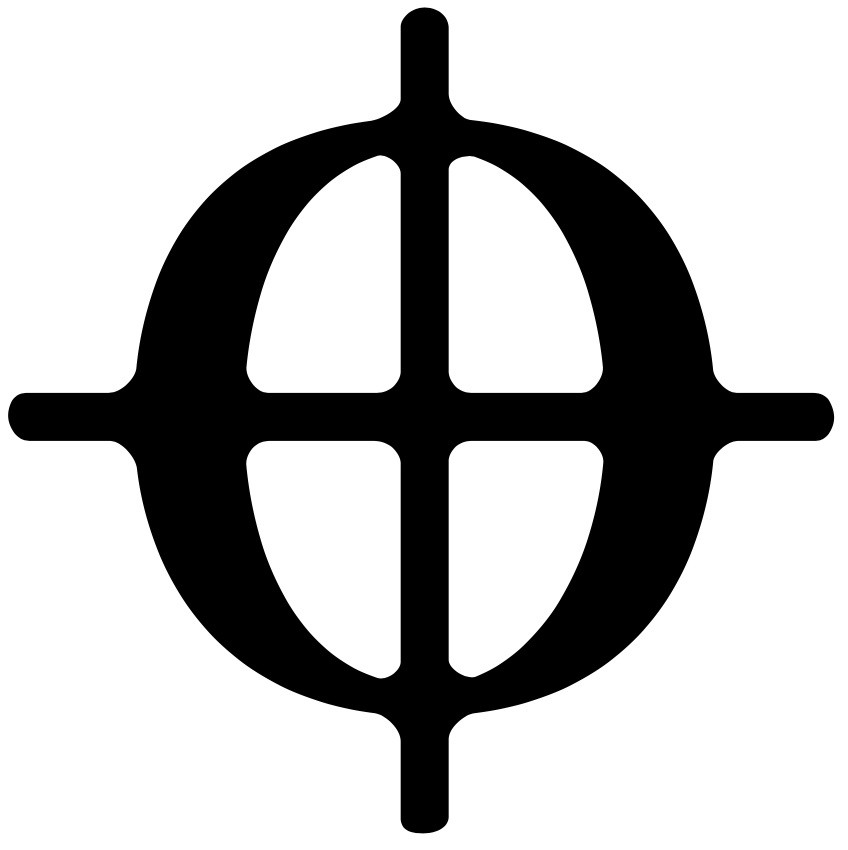
\includegraphics[scale=0.06]{damp.png} Indicates to \textbf{damp} the string with the \textbf{left hand}, removing as much pitch as possible. \\
\circled{4} Throughout the piece, a kind of \textbf{bariolage} appears, wherein the left hand maintains a \textbf{single chord} while the bow moves irregularly across the affected strings. For example, \\
\begin{center}
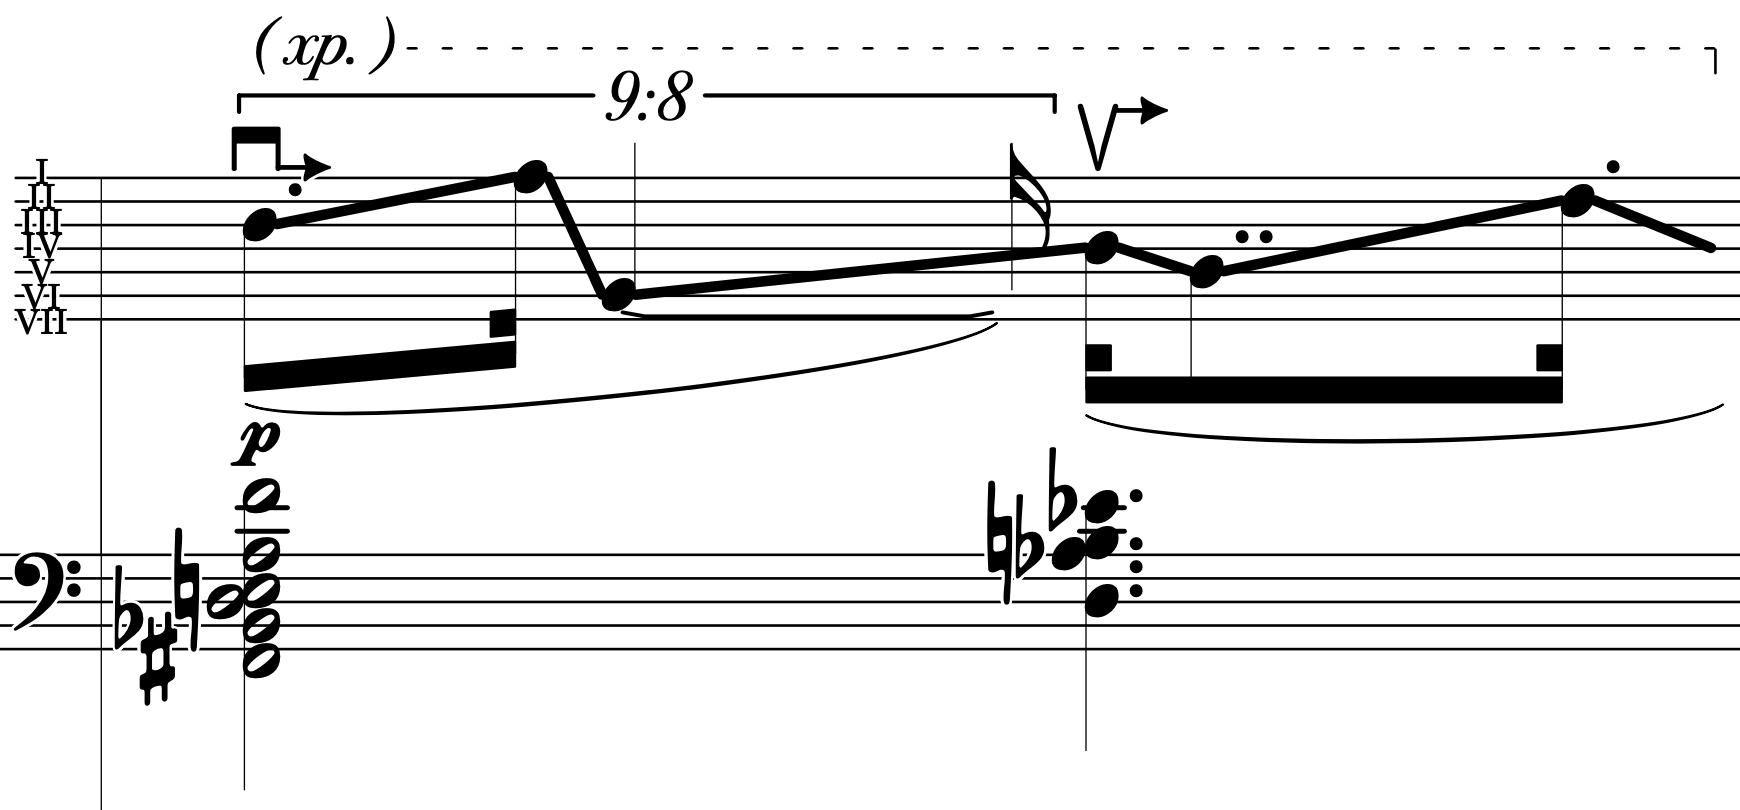
\includegraphics[scale=0.35]{bariolage.png} 
\end{center}
in the above excerpt, the right hand should draw the bow across the strings indicated by the top staff. The lines in between discreet arrival points should blur across all affected strings in the range, though still moving in a clear trajectory from one notated string to the next. 
\endgroup

\begingroup
\large \textbf{\circled{VI} THEORBO:} \\
\normalsize \circled{1} The interpreter should be equipped with a \textbf{plectrum}. \\

\pagebreak

\circled{2} Throughout the piece, a \textbf{rasgueado} is used wherein the amount of finger used, position on the string, and strings affected are specified. For example, \\
\begin{center}
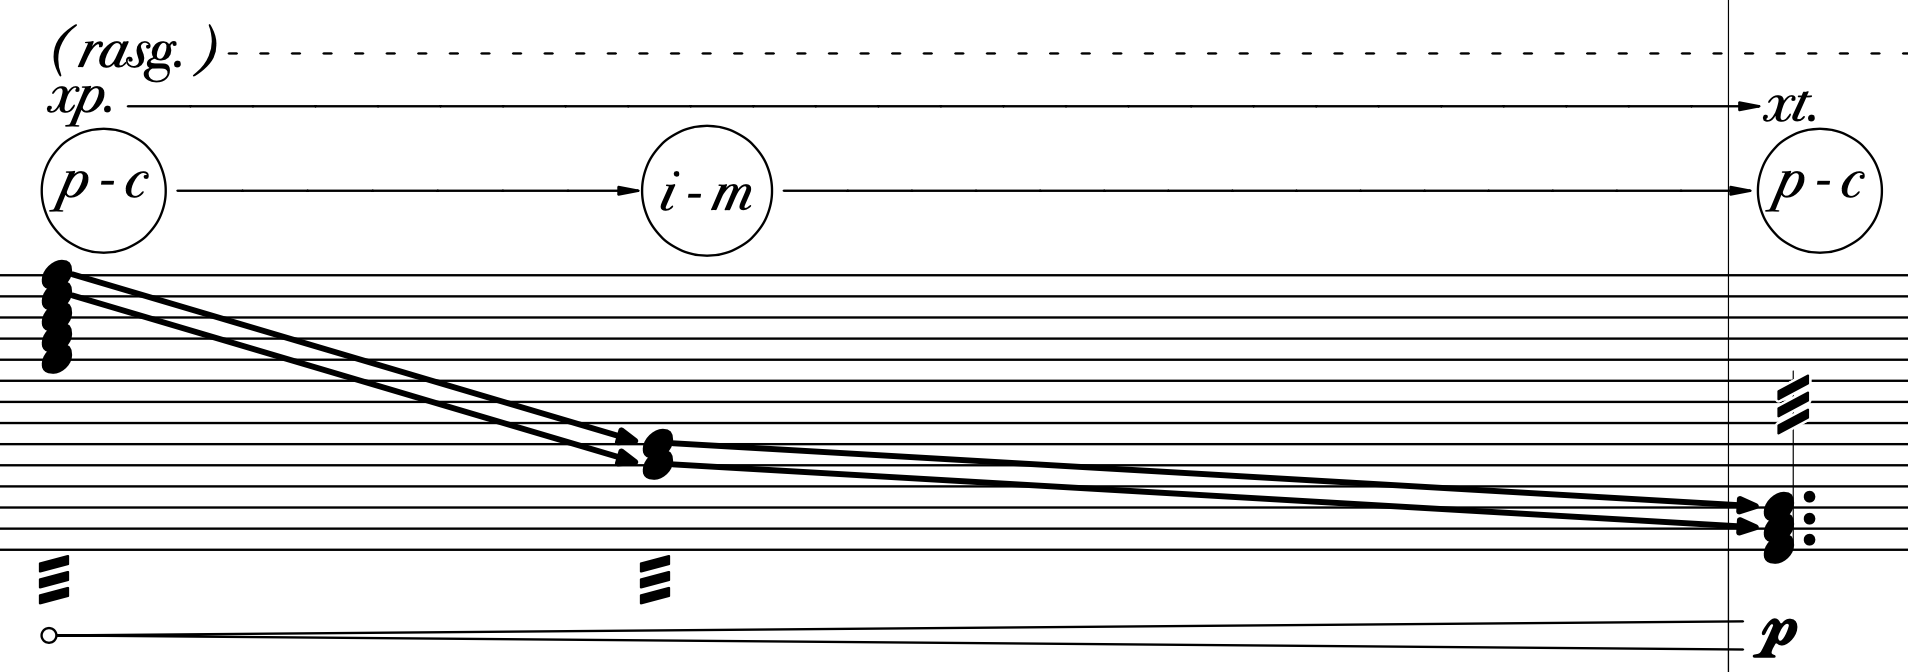
\includegraphics[scale=0.35]{rasgueado.png} 
\end{center}
in the above excerpt, the right hand should transition from using all fingers, to using only the index through middle fingers, and back all fingers, while moving the hand from extreme sul ponticello to extreme sul tasto. At the same time, the right hand should gradually change from affecting strings I-V, to strings IX-X, to strings XII-XIV. \\
\circled{3} In the excerpt below, \\ 
\begin{center}
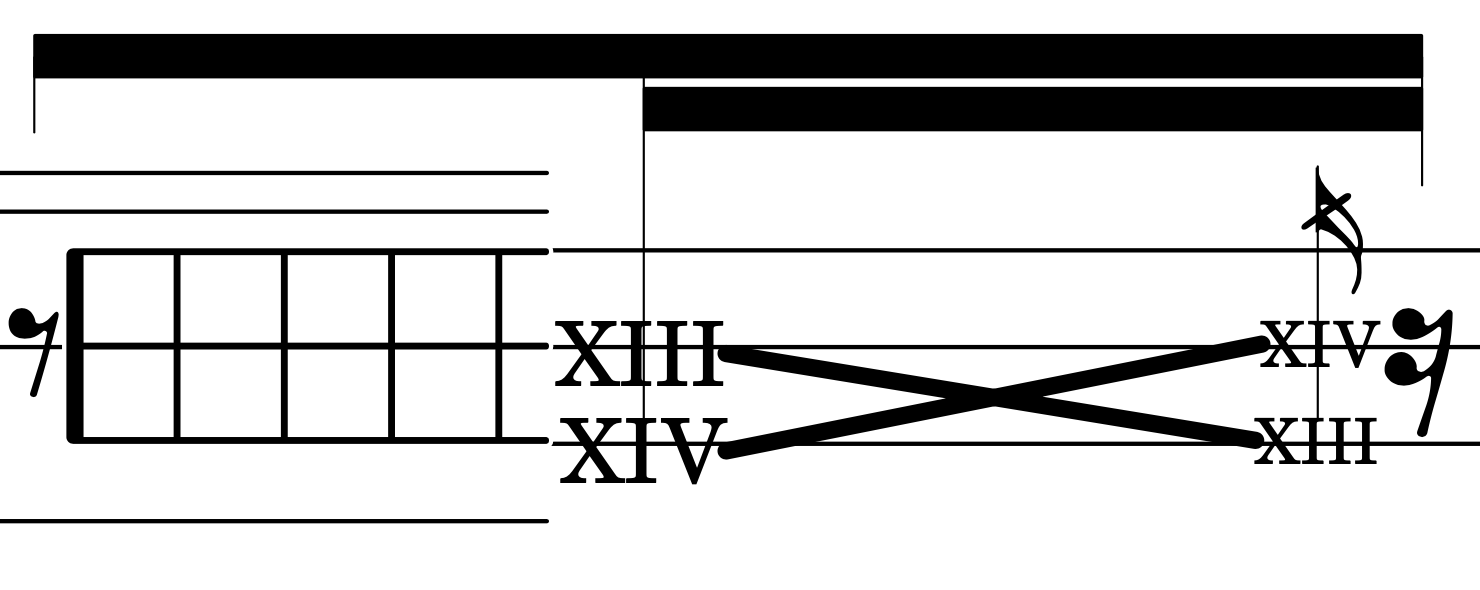
\includegraphics[scale=0.35]{twisting_excerpt_mm_3.png} 
\end{center}
the left hand should gradually pull strings XIII and XIV across one another in order to mute them and create a snare-like muting. At other points in the piece, as below:
\begin{center}
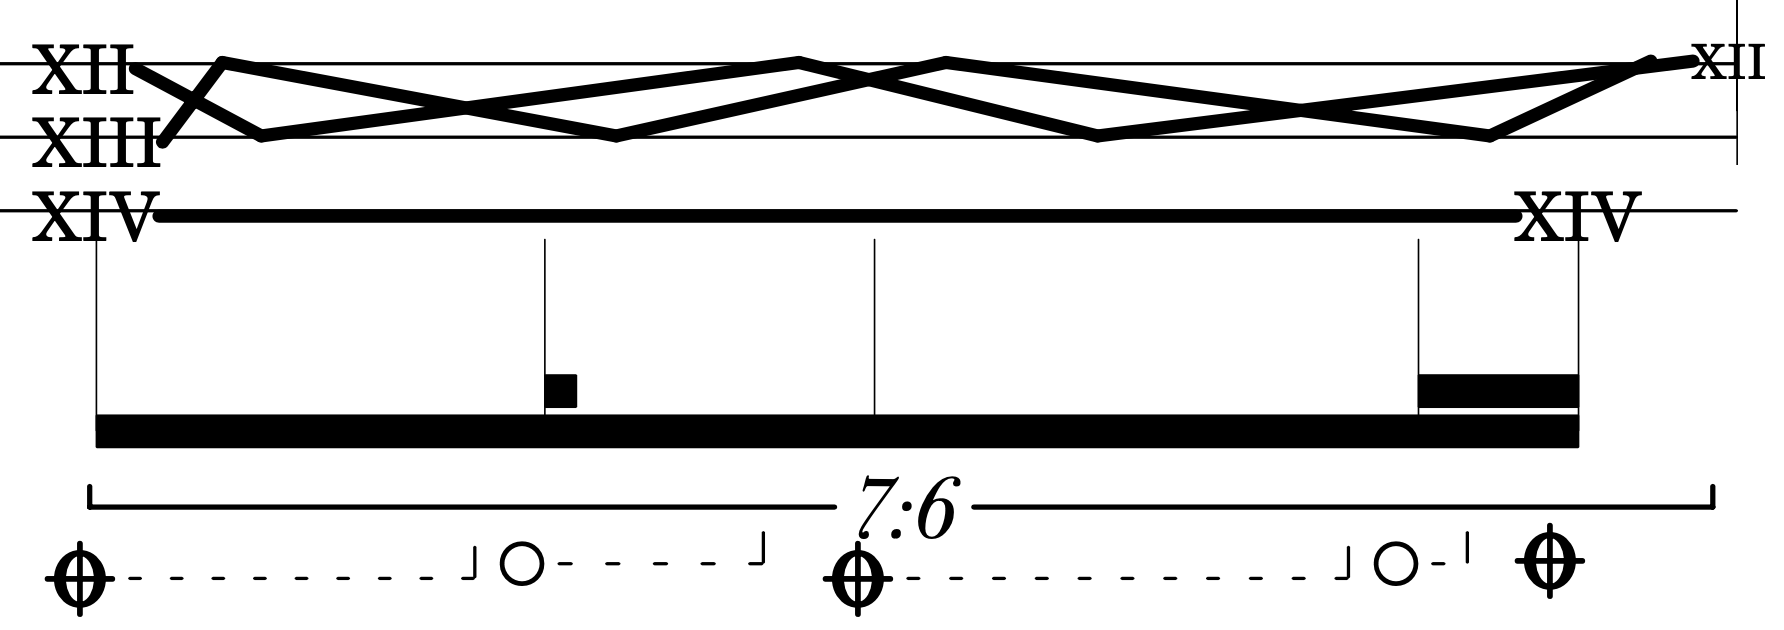
\includegraphics[scale=0.35]{twisting_with_mute.png} 
\end{center}
the same technique is performed on strings XII and XIII while a third finger only mutes and unmutes string XIV according to the rhythm below the staff. These excerpts are only from the left hand staff, as the techniques they use are always paired with some instruction in the right hand, usually a rasgueado. 
\endgroup

\end{document}